\documentclass[11pt,a4paper]{article}
\usepackage[top=22mm, bottom=22mm, left=22mm, right=22mm]{geometry}
\usepackage{amsmath, amssymb}
\usepackage{parskip}
\usepackage{enumitem}
\usepackage{hyperref}
\usepackage{xcolor}
\usepackage{graphicx}
\usepackage{geometry}
\geometry{margin=1.in}

\pagestyle{empty} % Remove page number

\begin{document}

\begin{center}
    {\LARGE \textbf{Executive Summary}} \\[1.5mm]
    
    {\Large Pricing Exotic Options using Stochastic Calculus, PDEs, and Monte Carlo Simulations} \\[2mm]
    
    \textbf{Ajay Singh} \\
    \texttt{ajay.s.works@gmail.com} \\
    June 2025
\end{center}
\vspace{3mm}
\noindent
\textbf{Overview:}
This project presents a unified computational framework for pricing exotic financial derivatives, such as Asian and barrier options, integrating stochastic calculus, Monte Carlo simulations, and finite difference PDE methods. We benchmark each method's accuracy, convergence, and runtime on realistic market scenarios.

\vspace{1mm}
\noindent
\textbf{Key Features:}
\begin{itemize}[leftmargin=10pt, itemsep=0pt, parsep=0pt]
    \item Modular Python implementation: Black-Scholes, Monte Carlo, Crank-Nicolson PDE.
    \item Full support for vanilla and exotic options, with variance reduction (Sobol, control variates).
    \item Comparative plots: convergence, runtime, accuracy, and Greeks for each method.
    \item Open-source code: \href{https://github.com/ajayworks/Pricing_Exotic_Options}{github.com/ajayworks/Pricing\_Exotic\_Options}
\end{itemize}

\vspace{1mm}
\noindent
\textbf{Results:}
\begin{itemize}[leftmargin=10pt, itemsep=0pt, parsep=0pt]
    \item Analytical and numerical methods are consistent for vanilla options.
    \item For exotic options, MC and PDE are benchmarked against reference solutions.
    \item MC variance reduction (Sobol sequences, control variates) substantially boosts accuracy.
    \item PDE solver is stable and accurate for path-dependent payoffs.
    \item Greeks (sensitivities) computed for risk management and hedging.
\end{itemize}
\begin{center}
    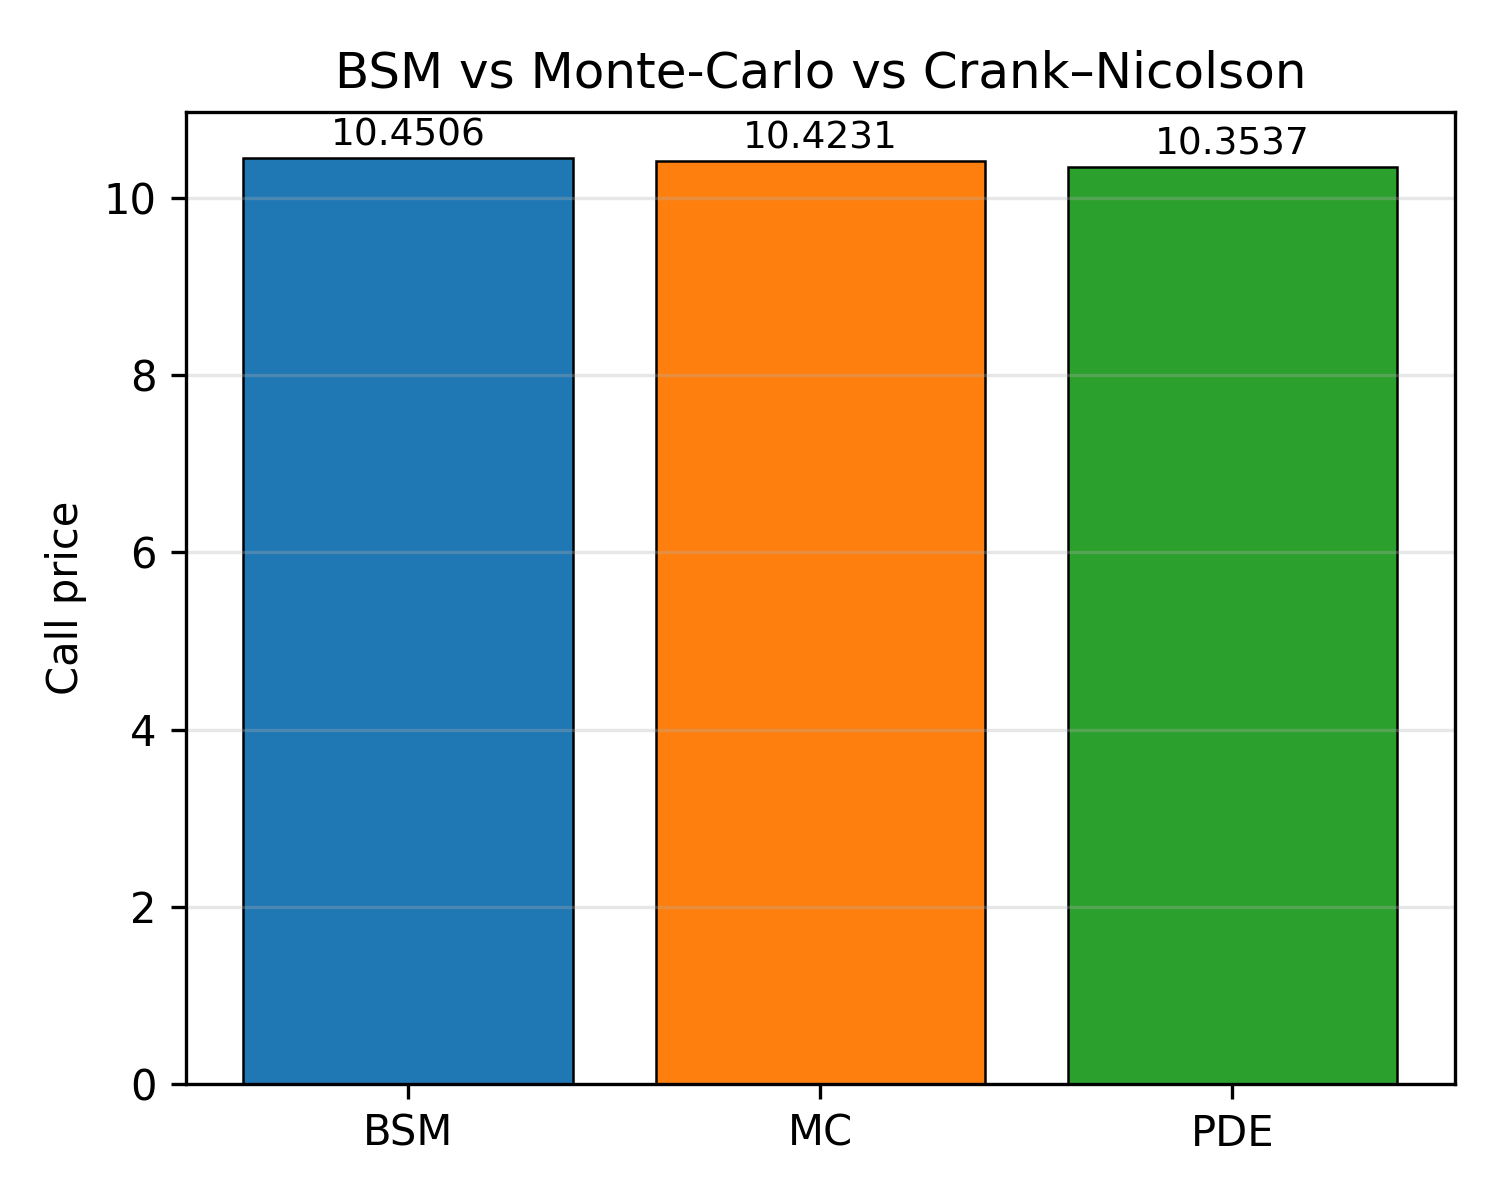
\includegraphics[width=0.6\textwidth]{../plots/BSM_MC_CN_comparison.png}
    
    \textit{\small Figure: BSM vs Monte Carlo vs Crank-Nicolson (PDE) pricing for a European call option.}
\end{center}
\vspace{1mm}
\noindent
\textbf{Impact:}
This project lays a robust foundation for research and professional quantitative finance. The modular approach facilitates extensions to American-style options, stochastic volatility models, and machine learning-based pricing. Future work includes calibration to real market data and backtesting.

\end{document}